%%%%%%%%%%%%%%%%%%%%%%%%%%%%%%%%%%%%%%%%%%%%%%%%%%%%%%%%%%%%%%%%%%% 
%                                                                 %
%                           INLEIDING                             %
%                                                                 %
%%%%%%%%%%%%%%%%%%%%%%%%%%%%%%%%%%%%%%%%%%%%%%%%%%%%%%%%%%%%%%%%%%% 


\chapter{Ontwerpproces}

In dit hoofdstuk worden de ondernomen stappen besproken bij het ontwerpen van een interface die kristalstructuren, in de vorm van een CIF-bestand, kan visualiseren in Blender. Een meer gedetailleerde beschrijving van dit proces kan worden gevonden in hoofdstuk vier, hier wordt ook dieper ingegaan in de installatie van de twee externe programma's, OpenBabel en PyCIFRW, die zullen besproken worden in dit hoofdstuk. De eerste sectie beschrijft hoe de inwendige symmetrie een probleem vormt bij het visualiseren van kristallen, wat het programma OpenBabel doet en hoe het gebruiken hiervan een oplossing biedt op dit probleem.
In de tweede sectie zal worden uitgelegd hoe, met behulp van een parser, een programma in Python kan geschreven worden dat de gegevens uit een CIF-bestand kan omzetten in verwerkbare data en deze opslaat in geschikte datastructuren.


\section{Omvormen van het invoersbestand}

\subsection{Symmetrieoperaties in het CIF-formaat}
Zoals in sectie 2.1.5 van deze tekst staat beschreven kan een kristal worden beschreven aan de hand van een aantal parameters en een lijst van elementen. Dit kan ook gezien worden in het CIF-bestand van Chaziet[Bijlage B] waar slechts vijf atomen worden beschreven terwijl het eenheidskristal in het totaal uit 150 atomen bestaat. Dit is erg handig aangezien er dertig keer zo weinig atomen moeten worden beschreven. In dit onderzoek vormt dit echter een probleem. Om een kristal te tekenen dient natuurlijk de positie van elk element gekend te zijn.
\par
Aan de hand van de ruimtegroep en de centering van het kristalrooster kunnen alle symmetrieoperaties worden verkregen. Deze symmetrieoperaties zijn in het CIF-formaat reeds gegeven in het blok \textit{\_symmetry\_equiv\_pos\_as\_xyz} als een lijst van fractionele coördinaten. Vanuit deze symmetrieoperaties kunnen de posities van elk element in het kristal berekend worden. Er dient rekening gehouden te worden met de mogelijkheid dat één bepaald element aan de hand van verschillende berekeningen kan verkregen worden zodat dit niet meermaals wordt genoteerd, en later getekend. Het is mogelijk een functie te schrijven die de lijst van symmetrieoperaties ophaalt en vervolgens voor elk van deze symmetrieoperaties de positie van de elementen berekenen die ze representeren. Er bestaan echter reeds programma's die dit soort berekeningen kunnen doen, OpenBabel is hier één van.
\par
\subsection{OpenBabel}
OpenBabel is een open source chemische toolbox die gebruikt wordt om chemische data te zoeken, analyseren en te converteren.\citep*{OBAB1} Naast het converteren tussen een groot aantal chemische dataformaten kan OpenBabel ook binnen eenzelfde formaat data converteren. Deze functionaliteit laat onder andere toe de kristaldata van een CIF-bestand om te zetten naar data van datzelfde kristal met een andere ruimtegroep. Door de ruimtegroep aan te passen naar dat van P 1 zal er geen inwendige symmetrie meer bestaan, dit wil zeggen dat elk element dat beschreven wordt slechts op één plaats voorkomt. In plaats van een lange lijst van symmetrieoperaties zal elk element dat gevormd kan worden door deze operaties in het blok met de atoombeschrijvingen komen te staan.   
\par
De broncode van OpenBabel staat vrij beschikbaar op hun GitHub pagina.  Hiernaast is het ook mogelijk de GUI-versie van OpenBabel te downloaden door de installatie-instructies te volgen die te vinden zijn op hun officiële webpagina.\citep*{OBAB1}   
\par
\begin{figure}[h]
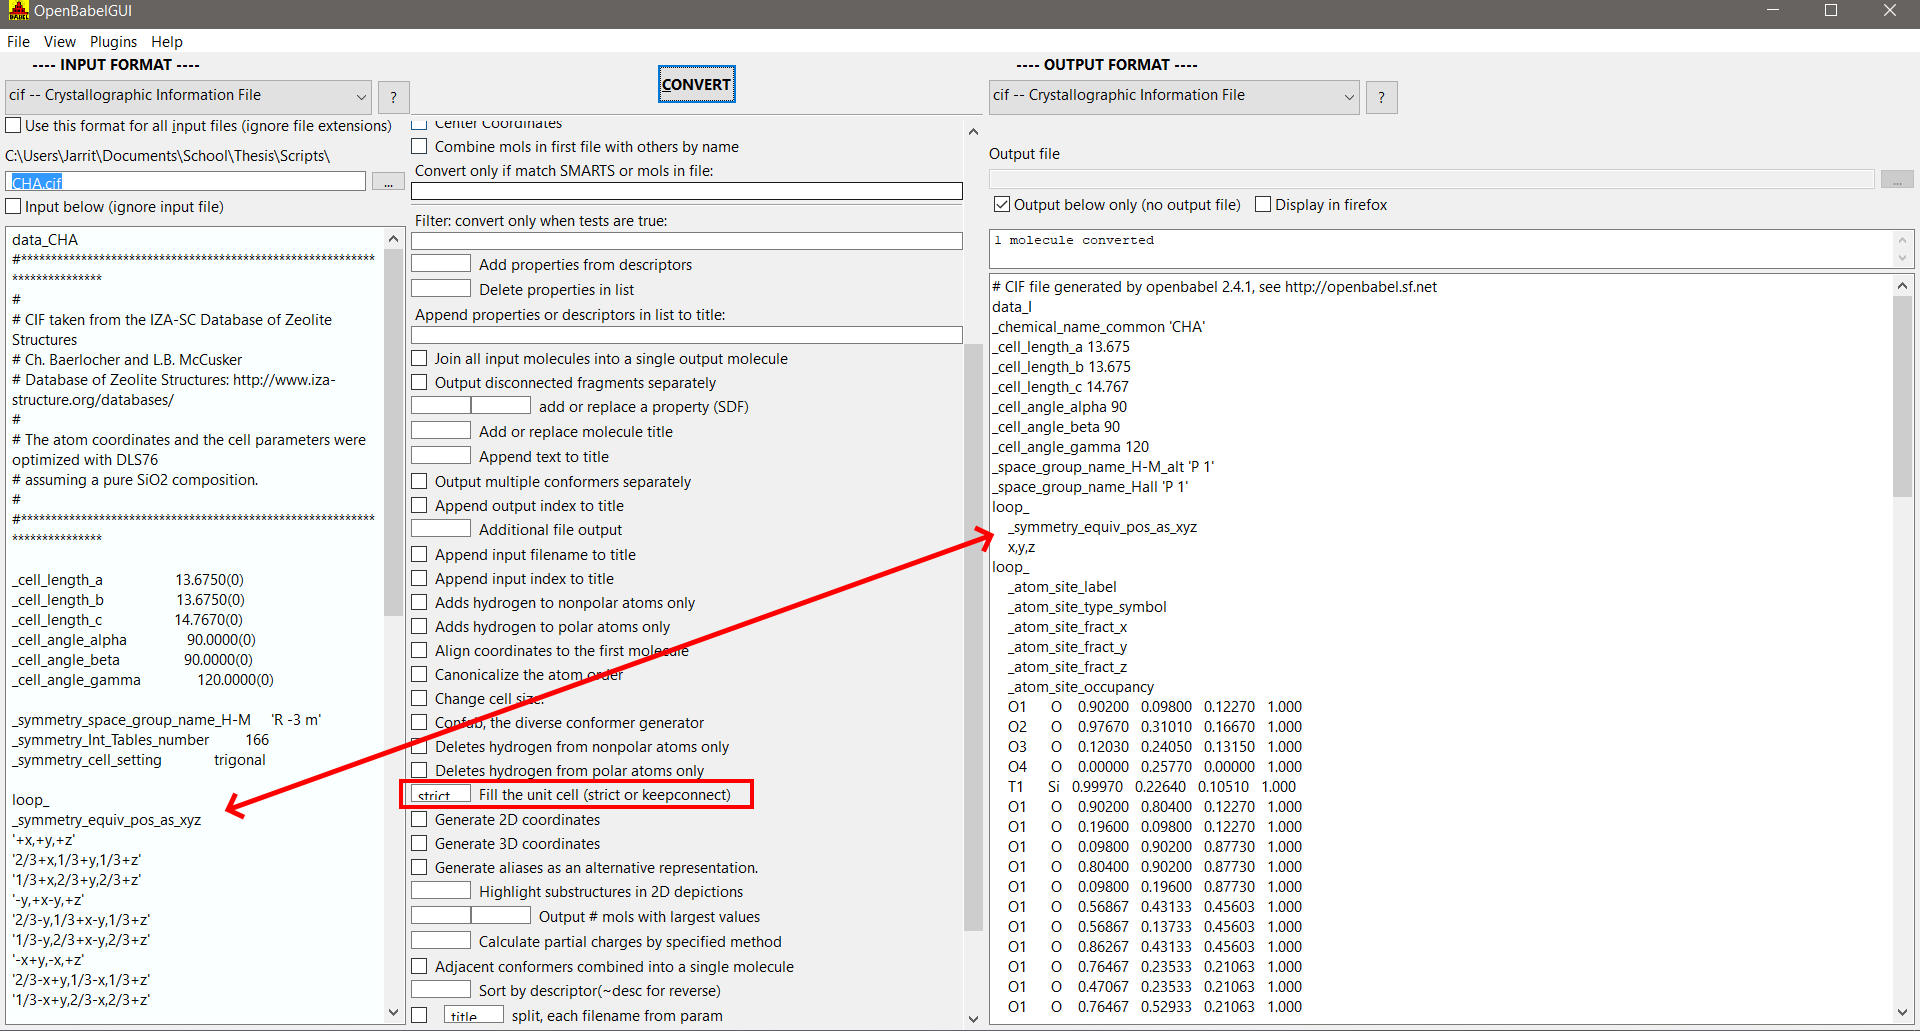
\includegraphics[width=\textwidth,keepaspectratio]{OpenBabelGUI.png}
\caption{Conversie van ruimtegroep met OpenBabel GUI}
\end{figure}
\par
In figuur[3.1] wordt de GUI van OpenBabel afgebeeld. In de linker- en rechterkolom van dit venster staan de in- en uitvoer van het programma en hun formaat. In de middelste kolom kunnen verschillende soorten van conversies worden aangeduid. In het geval van de afbeelding zijn zowel in- als uitvoer in het CIF-formaat en staat het \textit{Fill the unit cel}-vakje op \textit{strict}. Deze opties zorgen ervoor dat het invoerbestand zal worden omgezet naar een ander CIF-bestand maar ditmaal zonder symmetrieoperaties, wat duidelijk wordt bij het bekijken van de twee buitenste kolommen. Bij dit voorbeeld is er maar een optie aangeduid, er zijn nog een groot aantal erg handige keuzemogelijkheden maar deze komen voorlopig niet aan bod.
\par
Hoewel de OpenBabel GUI het converteren van data erg eenvoudig en overzichtelijk maakt, zou het niet erg efficiënt zijn dat dit proces manueel moet worden gedaan voor elk kristal. Deze software kan echter ook vanuit een terminal worden uitgevoerd, wat, in combinatie met de subprocess module van python, de kristallografische interface toelaat deze conversie automatisch te laten verlopen. In hoofdstuk vijf wordt dit in meer detail uitgelegd.
\par     
\section{Van CIF naar py}

\subsection{Ontwerpen van datastructuren}
Nu het CIF-bestand naar een meer bruikbaar formaat is omgezet, is er nood aan datastructuren waarin de informatie kan geparsed worden. Zo een datastructuur noemt men een klasse en het werken hiermee wordt object georiënteerd programmeren genoemd. Enkele voordelen dat dit biedt over de klassieke, imperatieve methode van programmeren, zijn overzichtelijkheid, herbruikbaarheid van klassen en een extra laag van veiligheid doordat de data niet rechtstreeks kan worden aangepast.
\par
Het inlezen van de data wordt in drie klassen gedaan. Een eerste klasse, \textit{Cell}, die informatie bevat over het kristalrooster, waaronder de roosterparameters. Deze data-elementen worden ook wel de attributen van een klasse genoemd. Een tweede klasse, \textit{Atom}, die de fractionele coördinaten van het atoom bevat en welk element het voorstelt. De derde klasse, \textit{Crysdata}, overkoepelt voorgaande klassen in de zin dat deze naast de naam van het kristal ook één object van de klasse \textit{Cell} en een lijst van objecten van de klasse \textit{Atom} bevat. Hiernaast bezit elke klasse ook de methode, \textit{printout()}, die de data van de klasse op een nette manier weergeeft op de terminal, en de methode \textit{draw()} die later gebruikt wordt om het object te tekenen in Blender. Methodes zijn functies die op een object van een klasse kunnen worden opgeroepen.  In Figuur[3.2] worden de onderlinge verhoudingen van deze klassen verduidelijkt, dergelijke figuur wordt een klassendiagramma genoemd, en geeft de algemene opbouw van een programma aan de hand van de gebruikte attributen, methodes, modules en hun onderlinge relaties. Uit dit diagram kan er geïnterpreteerd worden hoe de data uit het CIF-bestand met behulp van de PyCIFRW-parser zal worden ingelezen in de drie eerder genoemde klassen.

\begin{figure}[h]
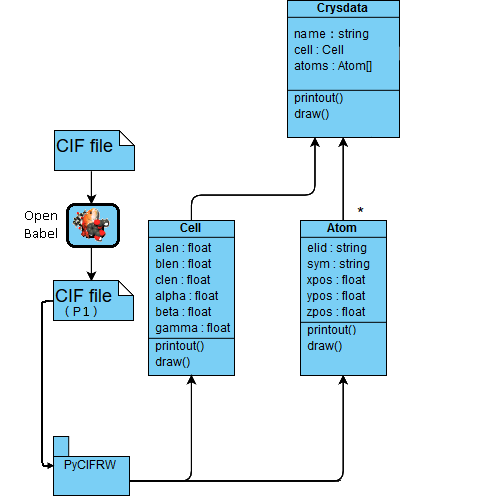
\includegraphics[scale=0.7]{ClassDiagramEz.png}
\caption{Vereenvoudigd klassendiagramma van het programma}
\end{figure}

\subsection{Inlezen van CIF-bestanden}
In de vierde sectie van hoofdstuk twee van deze tekst wordt het nut en de werking van een parser besproken. Er wordt ook gekeken naar twee bestaande programma's die in staat zijn CIF-bestanden te parsen en waarom PyCIFRW de voorkeur krijgt in dit onderzoek.
\par
Door de module \textit{CifFile} te importeren kunnen de schrijf- en leesfuncties van PyCIFRW worden opgeroepen in het programma. Nu kan het bestand, dat eerder werd omgezet met behulp van OpenBabel, worden geparsed. De geparsede data zal in de vorm van een soort dictionary ter beschikking zijn. Een dictionary is een python structuur die bestaat uit een lijst van sleutels, \textit{keys}, en hun corresponderende waarden, \textit{values} genoemd. De data kan verkregen worden door de dictionary op te roepen met een bepaalde sleutel.
\par
De sleutels van de dictionary die de PyCIFRW parser aanmaakt stemmen overeen met de namen die te vinden zijn in het CIF-bestand zelf. Op deze manier kan de data dus bekomen worden die vervolgens in de klassen worden ingevuld.

\section{Tekenen in Blender}
\subsection{Berekenen van de conversiematrix}
Voor er kan getekend worden dienen alle fractionele coördinaten omgezet te worden  naar hun overeenkomstige orthogonale waarden. Dit wordt gedaan aan de hand van een functie die de conversiematrix berekend op de methode die beschreven wordt in de eerste sectie van hoofdstuk twee. Deze matrix wordt opgeroepen wanneer de conversie tussen fractioneel en orthogonaal moet gebeuren.

\subsection{Omkadering van de eenheidscel}
Het eerste en meest eenvoudige object dat getekend wordt zijn de randen van de eenheidscel. Deze acht ribben worden in feite reeds beschreven door de roosterparameters van het kristal. Het tekenen van deze wordt gedaan door de coördinaten van de hoekpunten te berekenen, en tussen elk hoekpunt en zijn drie 'buren' een ribbe te tekenen. Zo een ribbe wordt getekend als een cilinder aangezien lijnen geen volume bezitten en niet als vormen beschouwd worden in Blender. 
\par
Voor het berekenen van de hoekpunten is er niet echt nood aan de conversiematrix. Deze kunnen op een goniometrische manier berekend worden met behulp van de lengte van de ribben en hun onderlinge hoeken. Het is echter eenvoudiger de fractionele waarden van de hoekpunten te gebruiken aangezien elke coördinaat van zo een hoekpunt steeds een nul of een één moet zijn. Door de fractionele coördinaten met de conversiematrix om te zetten kunnen de orthogonale coördinaten van de hoekpunten verkregen worden. Ten slotten kunnen de cilinders getekend worden tussen deze punten. Door de alle cilinders die de omkadering vormen samen te nemen als één object wordt de uiteindelijke omkadering bekomen.
\par
\subsection{Atomen}
Vervolgens dient de eenheidscel opgevuld te worden met de atomen van het kristal. De lijst van alle elementen en hun positie binnen het kristal is te vinden als attribuut de klasse \textit{Crysdata}. Deze lijst wordt doorlopen en op elk element zal zijn methode \textit{draw()} worden opgeroepen. Deze methode zal met behulp van de conversiematrix de orthogonale coördinaten van het atoom berekenen. Met behulp van een dictionary die voor elk elementen de straal van het atoom bevat kan vervolgens een bol getekend worden met de correcte afmetingen. En ten slotte, aan de hand van een andere dictionary die de kleur van de elementen bevat, krijgt deze bol een kleur toegekend. 
\par
\subsection{Atoombindingen}
Het programma laat ook toe bindingen tussen atomen te tekenen, op basis van hun onderlinge afstand. De gebruiker kan een variabele aanpassen die bepaalt hoe groot de afstand tussen twee atomen maximaal mag zijn, zodat de binding tussen deze gemaakt zal worden.
\par
Het programma zal vervolgens weer de lijst met atomen doorlopen en voor elk atoom de afstand tussen zichzelf en alle andere berekenen. In het geval dat deze onderlinge afstand kleiner is dan de door de gebruiker gekozen waarde, zal er een binding aangemaakt worden. Het tekenen van een binding zou op een gelijkaardige manier kunnen gedaan worden als het maken van de omkadering, er wordt echter een andere manier gebruikt die de bindingen zal vasthechten aan het atoom. Dankzij deze feature zal, wanneer de gebruiker een atoom versleept, het uiteinde van de binding vast blijven hangen aan het atoom. 
\par
Op Figuur[3.3] zijn de drie onderdelen van het getekende eenheidskristal te zien, eerst de omkadering, dan de atomen en ten slotte de bindingen tussen de atomen.
\begin{figure}[h]
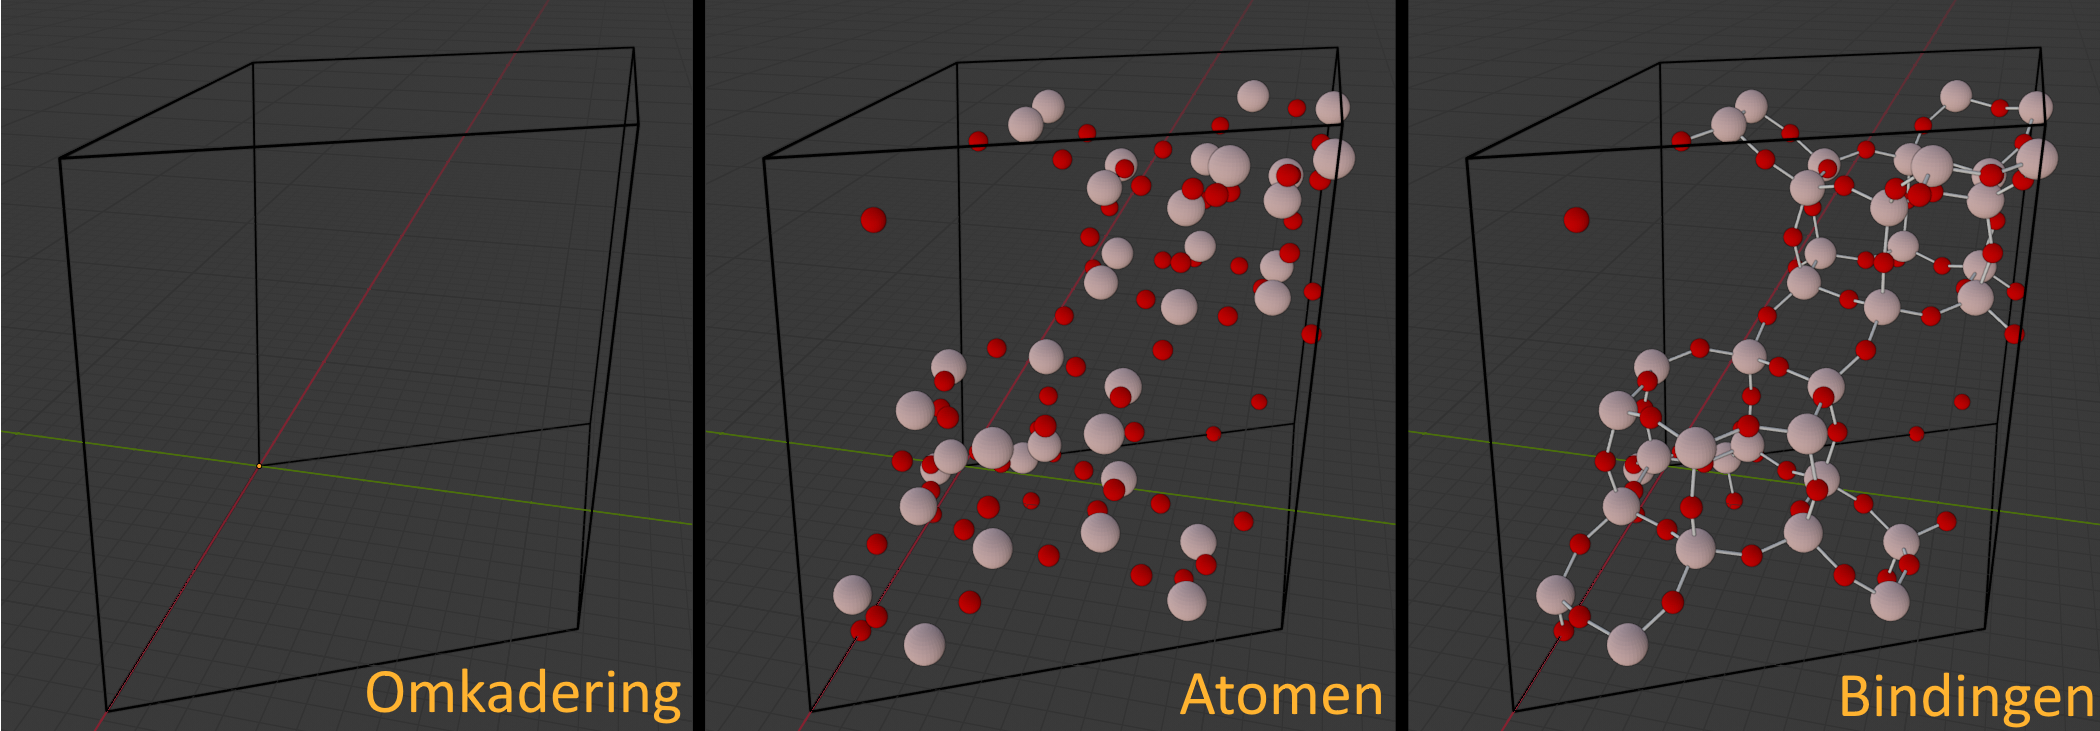
\includegraphics[width=\textwidth,keepaspectratio]{getekend.png}
\caption{De drie stappen in het tekenen van een kristal}
\end{figure}

\section{Creëren van een Blender add-on}

\subsection{Blender add-ons}
De laatste stap in het ontwerpproces is het aanmaken van een interface tussen de gebruker en het programma zodat de gebruiker op een eenvoudige manier zijn CIF-bestanden kan visualiseren. Blender laat toe zelf add-ons te creëren. Zo een add-on is een programma dat in de Blender interface kan worden opgeroepen door op de F3 toets de drukken, het is zelfs mogelijk een add-on een eigen venster te geven of in een reeds bestaand venster in te voegen.
\par
Het schrijven van een add-on kan worden gedaan in de Scripting omgeving van Blender, waar het meteen kan uitgevoerd worden of in een externe IDE zodat deze later kan worden geïnstalleerd. Een add-on hoeft slechts een keer geïnstalleerd worden en kan vanaf dan worden herladen door de \textit{Reload Scripts} functionaliteit uit te voeren in Blender. Op deze wijze kan een externe IDE gebruikt worden, welke veel handiger in omgang is dan de text editor van Blender zelf, terwijl de add-on constant kan getest worden na elke aanpassing van het script.

\subsection{Opbouw van een add-on script}
Een Blender add-on moet steeds een bestand bevatten met de naam \textit{\_\_init\_\_.py}, dit is het bestand dat Blender eerst zal uitvoeren wanneer de add-on wordt aangemaakt. In dit bestand staat steeds een header gedeelte dat \textit{bl\_info} heet. Deze variabele is een dictionary waarin de details van de add-on worden vermeld, waaronder de naam van de add-on, de versie van Blender waarvoor deze is gemaakt, de naam van de auteur en in welke editor omgeving deze add-on kan worden gebruikt. Een header is nog niet genoeg om een werkende aad-on te hebben, bij het uitvoeren van een add-on gaat Blender zoeken naar een \textit{register} methode. Deze functie zal telkens worden opgeroepen wanneer Blender de add-on zal inladen, in deze functie worden alle onderdelen van de add-on ingeladen. Deze onderdelen worden in de volgende secties verder beschreven. Wanneer de add-on wordt uitgeschakeld zal de \textit{unregister} methode worden opgeroepen welke het tegenovergestelde doet van de eerder beschreven \textit{register} methode.
\par
\subsection{Operatoren}
Operatoren, of \textit{operators}, zijn klassen in een add-on waarin de uitvoerbare elementen worden beschreven. Deze bevatten telkens hun eigen \textit{register} en \textit{unregister} methodes. In de \textit{register} methode worden de attributen van de operator beschreven, welke Blender zal aanmaken bij het inladen van de add-on. Deze attributen kunnen dan eventueel uit het geheugen worden verwijderd bij het uitvoeren van de \textit{unregister} methode wanneer de add-on wordt uitgeschakeld. 
\par
Een operator kan ook een \textit{execute} methode bevatten, deze methode zal worden opgeroepen wanneer deze operator in de add-on wordt uitgevoerd. In deze methode kunnen de attributen worden aangepast of ingelezen, kunnen andere functies worden opgeroepen of kan code staan die moet worden uitgevoerd zodra de operator wordt opgeroepen.
\par
In het programma worden twee operators aangemaakt. Eén operator heeft als functie een bestandsbrowser te openen waarmee de gebruiker het CIF-bestand kan selecteren dat moet worden gevisualiseerd. De tweede operator voert het hele script uit dat in dit hoofdstuk beschreven wordt, vanaf het converteren van het bestand met OpenBabel tot het tekenen van het kristal in Blender. Deze operatorklasse heeft een groot aantal attributen die de gebruiker kan aanpassen, waaronder enkele \textit{booleans} die kunnen aan of uitgezet worden, een \textit{float} die de maximal bindingdsafstand van de atomen bepaalt en twee \textit{enumarations} die de tekenwijze en de kwaliteit van het tekenen bepalen. Een enumeratie is een datastructuur die een verzameling is van symbolische namen, of leden, die gebonden zijn aan unieke, constante waarden. Binnen een enumeration kunnen de leden met elkaar worden vergeleken en kan er over de leden worden geïtereerd.\citep*{ENUM} Het nut van deze enumerations komt in de volgende sectie aan bod.

\subsection{Panelen}
Panelen, of \textit{panels} zijn klassen die als voornaamste functie het visualiseren van de add-on op het Blender scherm hebben. Een paneelklasse heeft enkele attributen die onder andere de naam van het paneel, in welk venster en in welk gebied de add-on wordt weergegeven. Ook deze klasse bevat een \textit{register} en \textit{unregister} methode, om het paneel te initialiseren. Hiernaast is er nog de \textit{draw} methode, waarin de lay-out van het paneel kan worden aangepast. Hiermee kunnen de attributen van de operatoren worden weergegeven zodat ze door de gebruiker kunnen worden aangepast. Booleans worden weergegeven als selectievakjes, getallen als schuifbalken en tekstvakjes en de eerder vernoemde enumeraties als een keuzelijst van de elemten die het bevat. Hiernaast kunnen er labels gemaakt worden waarin tekst kan worden afgebeeld en worden de operators als een drukknop weergegeven die hun \textit{execute} methode uitvoert wanneer de gebruiker op deze knop klikt.

 


 



  






